%%%%%%%%%%%%%%%%%%%%%%%%%%%%%%%%%%%%%%%%%%%%%%%%%%%%%%%%%%%%%%%%%%%%%%%%%%%%%%%%
% This chapter describes the analytics tools and views
%
% - Should rewrite comparison section, see pacivicVIS paper
%%%%%%%%%%%%%%%%%%%%%%%%%%%%%%%%%%%%%%%%%%%%%%%%%%%%%%%%%%%%%%%%%%%%%%%%%%%%%%%
\chapter{Enabling Analysis}
A comprehensive analytic system requires a variety of ways to manipulate and
looking at data. In this section we describe solutions for trend detection,
making comparisons and high level overview.
 

\section{Heatmap Perspective}
The heatmap widget has generic support for visualizing a time series data. It 
allows different time series to be interchanged within the heatmap itself, showing 
different perspectives. This was done to support the different types of
analytical tasks discussed in Chapter 3. These tasks, such as
finding seasonal trends of a component and finding the worst performing
component, are quite different, requiring a localized view showing how a
single component performed over time, and the other requires a very high level
view designed to draw out outliers.

    % === Figure === 
	\begin{figure} 
	 \centering  
	 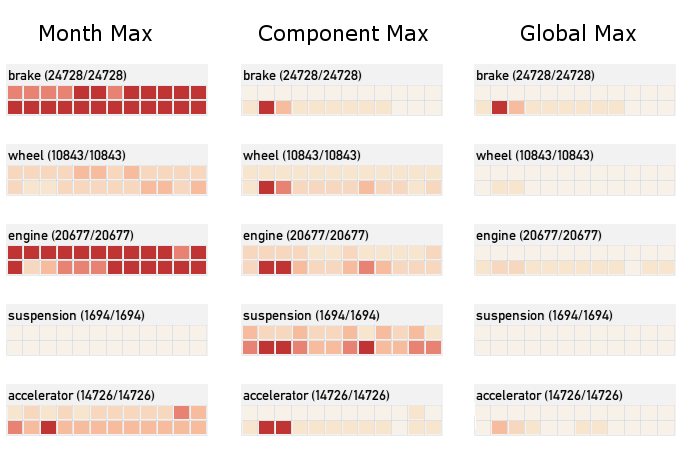
\includegraphics[width=\columnwidth]{heatmap_2.png}
	 %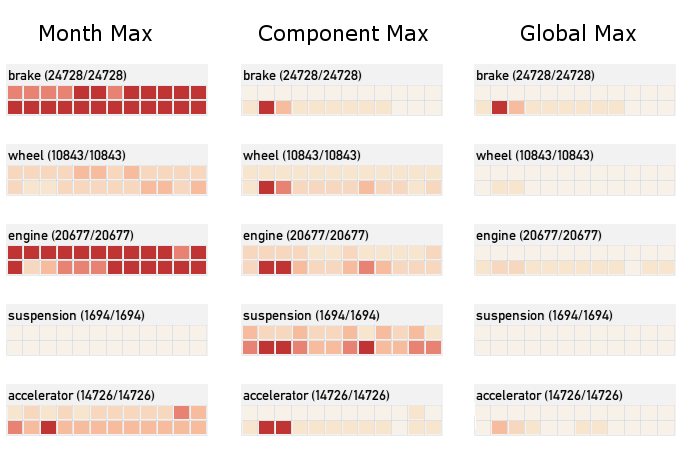
\includegraphics[scale=1.0]{heatmap_2.png}
	 \caption[Heatmap Perspectives]{The different heatmap perspectives. Left
	 displays the monthly perspective, centre displays the component perspective, and right displays the
	 global perspective}
	 \label{figure:heatmap}
	\end{figure}
	% ==============


Our visualization provides several different perspective views as shown in
Figure \ref{figure:heatmap}, all based on the occurrence score. The score of
each entity of each month is transformed by a divisor, which determines the
type of semantic we want to show. The available heatmap perspectives are listed below:

\begin{itemize} [noitemsep]
  \item Month-Max: A monthly perspective where the score of each month is 
  divided by the maximum score for that month amongst all components in the selected time.
  
  \item Component-Max: An entity-level perspective where the score of
  each month is divided by the maximum month score of the entity over the
  selected time. This is the default perspective in the system.
  
  \item Global-Max: A global perspective where the month score is divided by the
  maximum overall monthly score.
\end{itemize}
 
Here we illustrate how the perspective scoring works with an example of a time
over a period of three months: Suppose there are two entities, engine and brakes
and their occurrences scores over the three months are (1, 10, 100) and (10, 15,
20) respectively. In Table \ref{table:perspective} we show the entities' month
score under each perspective.

The monthly perspective draws out the
highest scored entity of each month, thus they are 10, 15 and 100 over the 3
months shown. Component view is localized for each entity, thus it is 100 for
engine entity and 20 for the brake entity over the 3 months. Finally global
perspective uses global maximum as the divisor, which is found in the engine
entity in the third month.
 
    % === Table ===
    \begin{table}[h]
	%\begin{tabular}{| l | lll | lll | lll | lll | 
	\begin{tabular}{| l | lll | lll | lll | 
	      } 
	   % Column Heading
	   \hline
	   %& \multicolumn{3}{|c|}{Score} 
	   & \multicolumn{3}{|c|}{Month Max} 
	   & \multicolumn{3}{|c|}{Component Max} 
	   & \multicolumn{3}{|c|}{Global Max} \\
	   
	   % Data 
	   \hline
	   Engine & %1 & 10 & 100 &       % Original
	            1/10 & 10/15 & 100/100 &      % Month
	            1/100 & 10/100 & 100/100 &    % Component
	            1/100 & 10/100 & 100/100 \\   % Global
	            
	   Brake &  %10 & 15 & 20  &      % Original
	            10/10 & 15/15 & 20/100 &      % Month
	            10/20 & 15/20 & 20/20  &      % Component
	            10/100 & 15/100 & 20/100 \\   % Global
	   \hline
	\end{tabular} 
	\caption{Sample perspective based scores} 
	\label{table:perspective}
	\end{table}
	% ============
  
Each of the perspectives above answers different questions and has its own
advantages and disadvantages. The month-max perspective allows people to compare 
component-to-component by month, but comparison against adjacent cells are 
meaningless because each cell uses a different base value. The component-max 
perspective is the opposite, it allows us to see trends with a single entity, 
but it does not allow comparison across components. Lastly, the global-max 
perspective is good at showing the outliers and supports both month-to-month 
and component-to-component comparisons, but it is difficult to see overall
trends because the outliers, if any, will dominate and push all non-outliers
into the same scoring bin.

To put the different perspectives in better context, we compile a list of sample 
questions that can be answered with these different perspective views:
\begin{itemize} [noitemsep]
  \item Month-Max: In month X, which vehicle component had the most complaints?
  \item Component-Max: Are there more braking problems in the summer months or
  the winter months? Are the number of complaints for wheels increasing or
  decreasing?
  \item Global-Max: What are the most unreliable vehicle components?
\end{itemize}

Going back to Figure \ref{figure:heatmap} as an example, one can make some
interesting observations. From the component view in the centre, a person can
see that there are two distinct outliers in the second and third months of the
second year, in particular, one can see the scores getting lower, then there is
a resurgence around July and August in the second year. Switching to the month-maxa
perspective, one can observe that during the two year period, the most
significant components seem to alternate between the brake and engine component,
with the sole exception of accelerator appearing in a single month. Lastly, the
global perspective yields three outliers, February and March from the brake entity
and February from accelerator entity. However, note the rest of the cells are
pushed into the lower brackets and not possible to detect any other trends.
 
The heatmap viewing perspective is at a global scope, thus a change in
perspective will affect all visible heatmaps. This keeps the interface
consistent and avoids viewers from switching to different modalities when they
shift their attention from one heatmap to another. The view switching mechanism
is realized as a drop-down control sitting atop the hierarchy widgets and shows
the currently selected viewing mode.



\section{Comparison}
Comparison mode allows people to compare entity occurrences across
two different subsets of the data. To select data to compare, we provide
two sets of filter widgets which can be used to specify manufacturer,
make, model and model year. Each set of filters specifies a query,
which we will call Q1 and Q2, and each query is assigned a colour,
which is used in the visualization. For example, we can compare
Honda Civic (Q1) to Toyota Corolla (Q2), or we can compare Ford
Focus (Q1) against all other Ford vehicles (Q2), by not fully specifying Q2.

Two separate measures are used to render the comparison view.
The \emph{contribution sum} is the aggregated component score from the two
query sets: it reflects the overall importance of the component by emphasizing
the most frequently occurring components matching Q1 and
Q2. The \emph{percentage difference} describes the relative frequencies of a
component, whether it occurs more frequently under Q1 or Q2 relative
to the total contributions from Q1 and Q2 respectively. The percentage
score is calculated as the component score divided by the total
contribution. Then the percentage difference follows as percentage
score Q1 minus percentage score Q2, with the sign and magnitude indicating
which query set has the stronger presence of that component.

We made the decision to use percentage-based comparisons because it
enables the comparison of query results of different sizes. For example, we can compare
a large manufacturer against a small manufacturer, even though we would expect the large 
manufacturer to have a greater number of complaint reports.
These scores are used to render the \threed view. Using the percentage
difference, the colour of the outline of a component indicates which
query set has the higher rate of complaints, and the opacity of the outline
indicates the strength of the difference. Using the contribution
sum, the standard hue and opacity encoding is used to indicate the
sum of the two query sets, giving an impression of the overall importance
of that component. Thus, a highly problematic component from
both queries will have a strong presence overall but with a faint outline,
while a lopsided but infrequently mentioned component will have
strong outline but barely visible interior colour.


    % === Figure ===
	\begin{figure}
	 \centering  
	 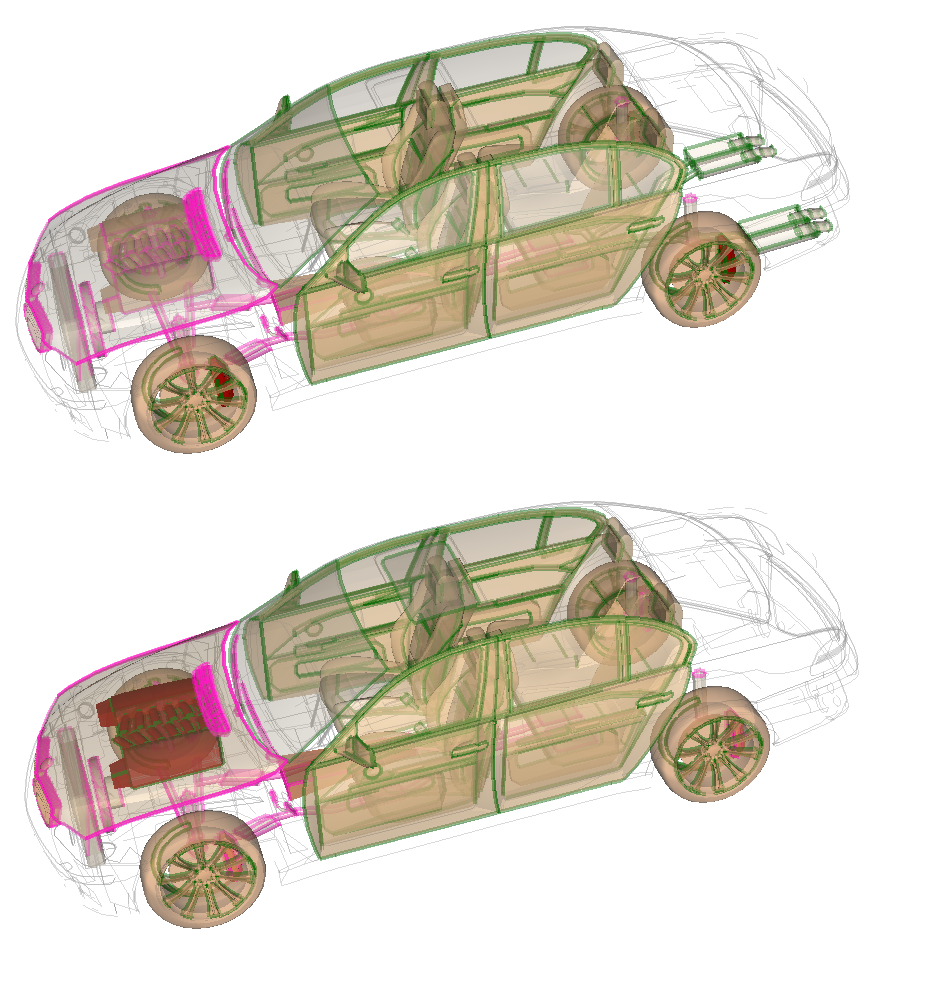
\includegraphics[width=\columnwidth]{comparison_3.png}
	 \caption[Comparison View]{Top: Vehicle A (pink) versus vehicle B (green), the
	 brake appears to be the dominant issue and B has the higher rate of complaints. Bottom:
	 Vehicle A (pink) versus vehicle C (green), the engine is the dominant issue
	 and B has higher rate of complaints.}
	 \label{figure:comparison}
	\end{figure}
	% ============== 
 
%As an example, see Figure \ref{figure:comparison}, where we compared Plymouth
%against both the Jeep and Chrysler. At a glance most parts remain the same
%with the exception of two outliers, Jeep appear to have a higher failure rate
%than Plymouth, and Dodge has a higher failure rate in brakes component. The
%overview could suggest that Plymouth is more reliable than both vehicles.

As an example, see Figure \ref{figure:comparison}. Vehicle A (pink) is compared
first against vehicle B at the top and vehicle C at the bottom. We can observed
that vehicle A has more complaints about the hood than both B and C. We can also
infer that B has serious problems with brakes and C has serious problems with
engine.
 
By default, comparison mode is turned off. It is activated when the viewer
switches the second hierarchy widgets from the ``None'' position to a valid
selection. Subsequent query modifications are carried out in comparison mode
until the selection is turned to ``None'' again.

%One limitation with this approach is our current usage of the total
%contributions to calculate the percentage scores. Our total contribution is in
%relations to the number of documents in the corpus, which may not be
%the best indication of the overall contribution.

 
 
 
\section{Aggregation}
By default, the system treats each object individually rather than object
groups. For example ``seatbelt'', ``backrest'' and ``seat'' are all processed
separately, even though they are logically under the group ``seat.'' This
setting allows people to isolate and identify low-level problems accurately. There
are times, however, when this level of information is unnecessarily detailed and
a higher level of abstraction is desirable.

    % === Figure === 
	\begin{figure}
	 \centering  
	 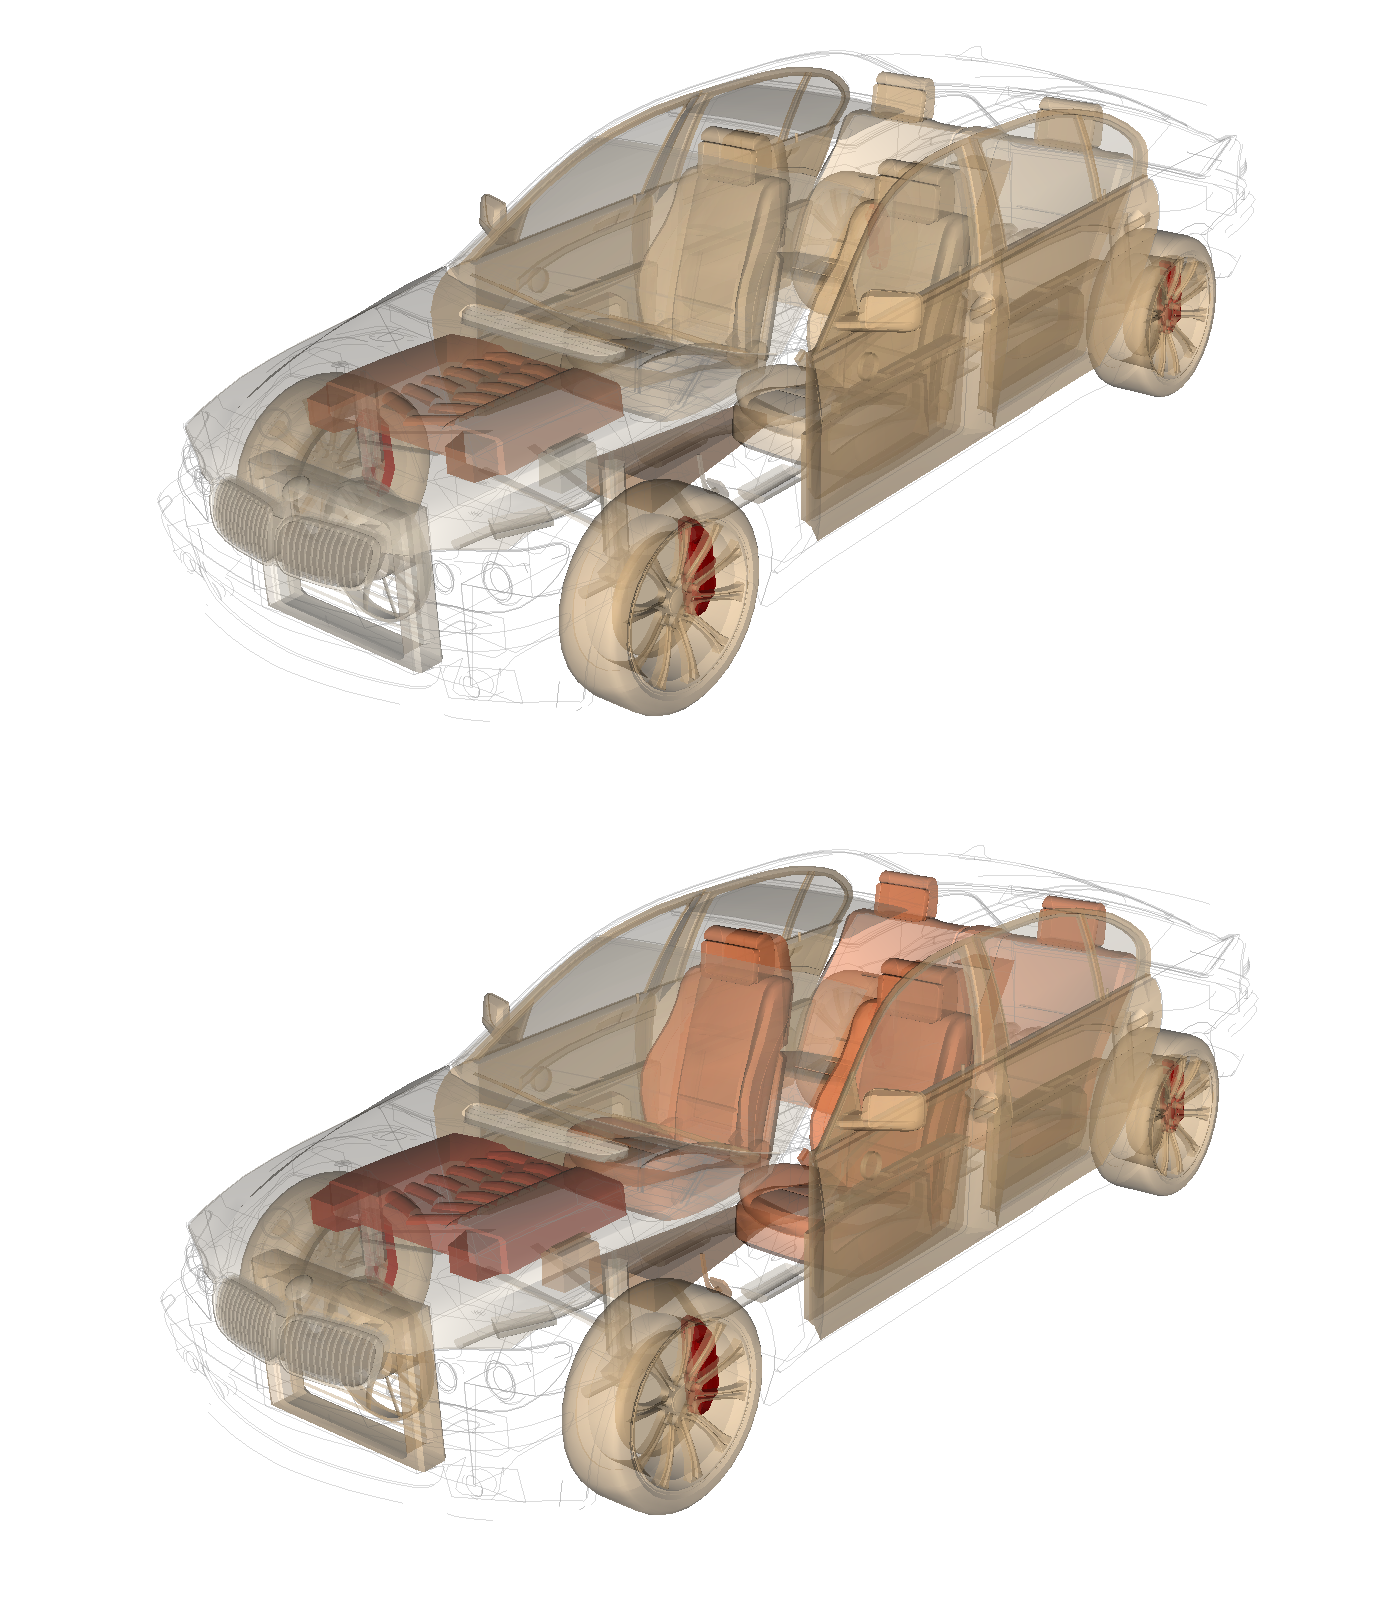
\includegraphics[width=\columnwidth]{aggregation2.png}
	 \caption[Aggregation View]{Top: Aggregation mode disabled. Bottom: Aggregation
	 mode enabled, note that the seat now appears more prominent in the visualization.}
	 \label{figure:aggregation}
	\end{figure}
	% ==============
	
Aggregation mode mimics the type of high level rating system found on consumers
review websites. When aggregation mode is enabled, individual objects, and their
scores are aggregated up to the first level entities in the keyword hierarchy. In our specific case, the 
first level are the major sub-systems in a vehicle. Aggregated components
responds to interaction events as a single group, thus, selecting the
``seatbelt'' will select the entire ``seat'' subsystem.

 
Figure \ref{figure:aggregation} shows a before and after illustration of using
aggregation mode. A default rendering is shown in the top portion, one can
only observe that brakes is the most severe out of all components. The bottom
shows the aggregated view, one can observe that on a higher level, the seat
subsystem is quite problematic.
 
Aggregation mode is enabled/disabled by a toggle switch located at the top
portion of the display interface. Aggregation mode is not exclusive, both aggregation
and comparison modes can be enabled at the same time, allowing viewers to make comparison
of major component systems.
